%!TEX program = xelatex

\documentclass[compress]{beamer}
%--------------------------------------------------------------------------
% Common packages
%--------------------------------------------------------------------------

\definecolor{links}{HTML}{663000}
\hypersetup{colorlinks,linkcolor=,urlcolor=links}

\usepackage[english]{babel}
\usepackage{pgfpages} % required for notes on second screen
\usepackage{graphicx}

\usepackage{multicol}


\usepackage{tabularx,ragged2e}
\usepackage{booktabs}

\setlength{\emergencystretch}{3em}  % prevent overfull lines
\providecommand{\tightlist}{%
  \setlength{\itemsep}{0pt}\setlength{\parskip}{0pt}}


\usetheme{hri}

\usepackage{remreset}% tiny package containing just the \@removefromreset command
\makeatletter
\@removefromreset{subsection}{section}
\makeatother
\setcounter{subsection}{1}

\newcommand{\source}[2]{{\tiny\it Source: \href{#1}{#2}}}

\usepackage{tikz}
\usetikzlibrary{mindmap,backgrounds,positioning}

\graphicspath{{figs/part1/}}

\title{ROCO318 \newline Mobile and Humanoid Robots}
\subtitle{Introduction}
\date{}
\author{Séverin Lemaignan}
\institute{Centre for Neural Systems and Robotics\\{\bf Plymouth University}}

\begin{document}

\licenseframe{github.com/severin-lemaignan/module-mobile-and-humanoid-robots}

\maketitle


\section{Module Overview \& Practicalities}
\begin{frame}{Module overview}

\begin{itemize}
\item Sensors for mobile and humanoid robots
\item Computer vision \emph{(Philip Culverhouse)}
\item Localisation
\item Planning and navigation
\item Bipedal robots
\item Robot control
\end{itemize}

\end{frame}

\begin{frame}{Availability}

    \begin{itemize}
        \item I have lots of time (2 hours) to deal with your queries in the laboratory sessions
        \item  Otherwise, the best thing to do is to email me first and see if I can sort out your query. If not then I will arrange a time to meet up with you.
        \item Don't forget – if you have any problems, or even if you are not sure about something - just email me

    \end{itemize}

    \begin{center}
        \texttt{severin.lemaignan@plymouth.ac.uk}
    \end{center}
\end{frame}

\begin{frame}{Registration}
        \centering
        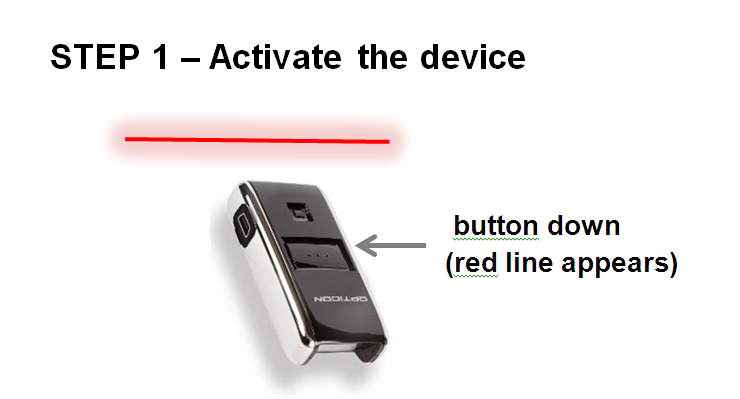
\includegraphics[width=0.4\linewidth]{registration1}
        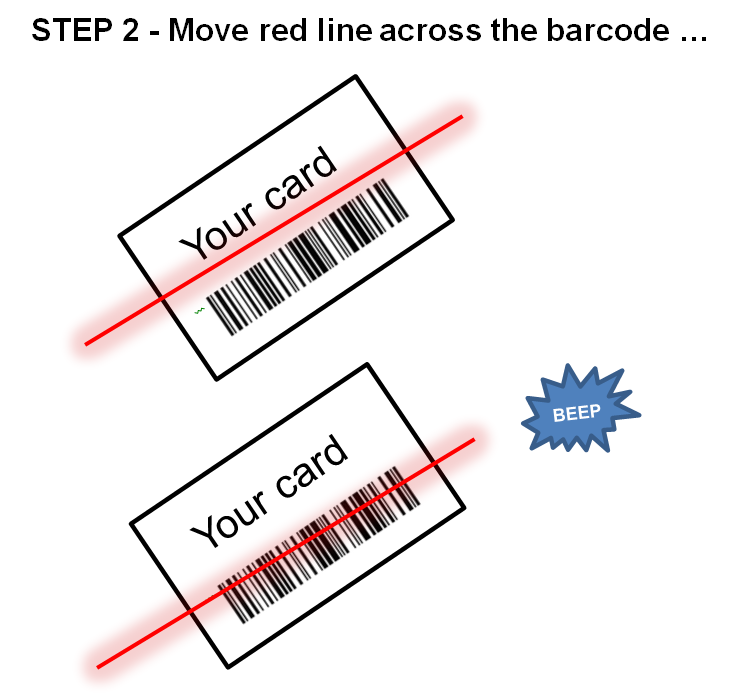
\includegraphics[width=0.4\linewidth]{registration2}
\end{frame}

\begin{frame}{Special needs}

    \begin{itemize}

    \item Anyone with dyslexia or any other special needs that requires any form
        of support during examinations and tests should email me immediately.

    \item Please do not ASSUME that I know of your condition. It takes the
        University some weeks to process data and forward it to the correct
            members of staff.

    \item Even if you are currently undergoing assessment, it is advisable to
        contact me and I will organize suitable support for you during your
            tests and exams.

    \item Contact me if any issues relating to harassment, inclusivity or if
        language/cultural difficulties arise.

    \end{itemize}
\end{frame}

\begin{frame}{This module: robotics syllabus}

\begin{itemize}
    \item<+-> \textbf{Week 1} -- Introduction
    \item<+-> \textbf{Week 2} -- Bipedal robots \emph{(with Martin Stoelen)}
    \item<+-> \textbf{Week 3} -- Sensors I
    \item<+-> \textbf{Week 4} -- Sensors II
    \item<+-> \textbf{Week 5} -- Kalman filtering
    \item<+-> \textbf{Week 6} -- Invited lecture: Brain-Computer Interfaces \emph{(with Dr. Claire Braboszcz)}
    \item<+-> \textbf{Week 7} -- \emph{no lecture}
    \item<+-> \textbf{Week 8} -- Wheeled locomotion
    \item<+-> \textbf{Week 9} -- Localisation and planning
    \item<+-> \textbf{Week 10} -- Robot control, ROS
    \item<+-> \textbf{Week 11} -- \emph{open!}
    \item<+-> \textbf{Week 12} -- Exam revision
\end{itemize}

\end{frame}

\imageframe[color=black, caption=github.com/severin-lemaignan/module-mobile-and-humanoid-robots]{github}

\begin{frame}{Robotics Labs -- from 02/10 to 03/11 (next 5 weeks)}
    \begin{alertblock}{Timetable mess-up}
        On Mondays: group 1 \\
        On Tuesdays: group 2 \\
        On Fridays: \textbf{everyone!}
    \end{alertblock}

          \begin{tabular}{@{}llll@{}}
                \toprule
                Day?                & Time? & Where?   & Who? \\ \midrule
                Monday -- Lab 3/\textbf{01} & 11:00--14:00     & SMB \textbf{302}  & Emmanuel \& Jake            \\
                Tuesday -- Lab 3/\textbf{02} & 09:00--12:00     & SMB 303b  & Emmanuel \& Jake          \\ \midrule
                Friday -- Lab 1 & 12:00--15:00     & SMB 303b  & myself \& Jake          \\ \bottomrule
            \end{tabular}


\end{frame}

\begin{frame}{Robotics Labs -- from 02/10 to 03/11 (next 5 weeks)}

    \begin{tabular}{@{}lll@{}}
        \toprule
        \bf Week           & \bf When      & \bf What \\ \midrule
        \bf 02/10 -- 06/10 & Mon/Tue    & \textcolor{hriSec1Dark}{\tt Humanoid robots}           \\
                           & Fri    & \textcolor{hriSec3Comp}{\tt Sensors project}           \\
        \bf 09/10 -- 13/10 & Mon/Tue    & \textcolor{hriSec1Dark}{\tt Humanoid robots}           \\
                           & Fri    & --           \\
        \bf 16/10 -- 20/10 & Mon/Tue    & \textcolor{hriSec1Dark}{\tt Humanoid robots}           \\
                           & Fri    & \textcolor{hriSec3Comp}{\tt Sensors project}           \\
        \bf 23/10 -- 27/10 & Mon/Tue    & \textcolor{hriSec3Comp}{\tt Sensors project}           \\
                           & Fri    & \textcolor{hriSec3Comp}{\tt Sensors project}           \\
        \bf 30/10 -- 03/11 & Mon/Tue    & \textcolor{hriSec3Comp}{\tt Sensors project}           \\
                           & Fri    & \textcolor{hriSec3Comp}{\tt Sensor demonstrations}           \\
    \end{tabular}


\end{frame}


\begin{frame}{Computer Vision Labs -- from 06/11 to 13/12}

          \begin{tabular}{@{}llll@{}}
                \toprule
                Day?                & Time? & Where?   & Who? \\ \midrule
                Wednesday -- Lab 2 & 09:00--11:00     & SMB 303b  & Phil           \\ \bottomrule
            \end{tabular}


\end{frame}



\begin{frame}{Assessment}

    \large
    \begin{itemize}
        \item Written exam: 70\%
        \item Coursework: 30\%
            \begin{itemize}
                \item 60\%: sensors project
                \item 40\%: computer vision project
            \end{itemize}
    \end{itemize}

\end{frame}


\begin{frame}{And what do I do?}

\begin{multicols}{2}

    \textbf{Cognitive robotics}

  Building robots and their artificial intelligence inspired on natural
  systems, such as developing children

    \textbf{Human-Robot Interaction}

  Building robots that can work alongside people, using social cues that
  people use to communicate

    \begin{center}
        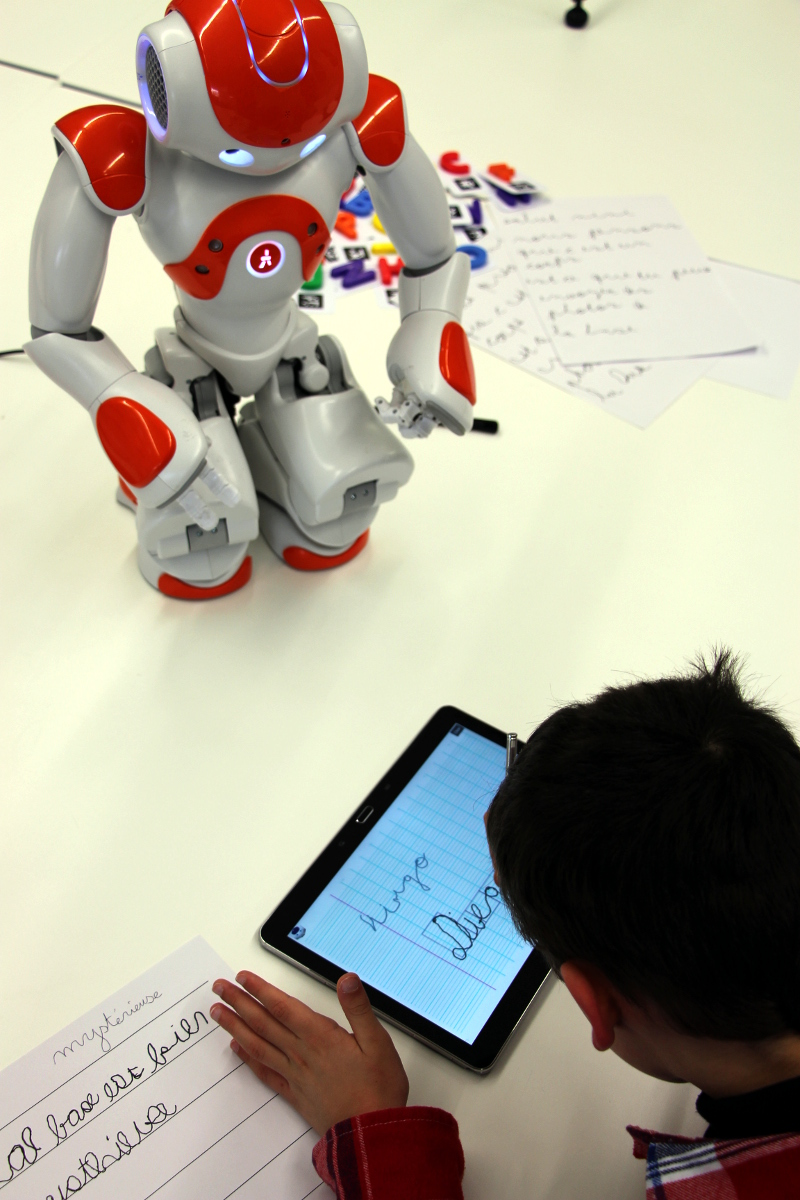
\includegraphics[width=0.8\linewidth]{cowriter}
    \end{center}

\end{multicols}
\end{frame}

\section[]{"Homework"}


\begin{frame}{"Homework"}
    \begin{itemize}
        \item<+-> Thinker with hardware and software!
        \item<+-> \textbf{Write code}, a lot of code -- preferably Python and C++ \\
                I am happy to answer code-related questions
        \item<+-> Invest \textsterling 30 and get a Arduino/RaspberryPI starter kit (like the \href{https://www.amazon.co.uk/s?merchant=A3DM8VCGJL5PKR&fallThrough=1}{Freenove ones})
        \item<+-> \textbf{Make it fun}: come up with \textbf{small, rewarding projects} -- Tetris anyone?
        \item<+-> \textbf{Install Linux} (and use it!) -- alongside Windows as a dualboot, or inside a VM
        \item<+-> Get involved in an \textbf{open-source project}

    \end{itemize}
\end{frame}


\section[]{That being said...}

\imageframe[scale=1]{pepper-robot}

\section[Pepper demo]{What have we seen so far?}

\begin{frame}[plain]

    \begin{multicols}{2}

        \begin{center}
            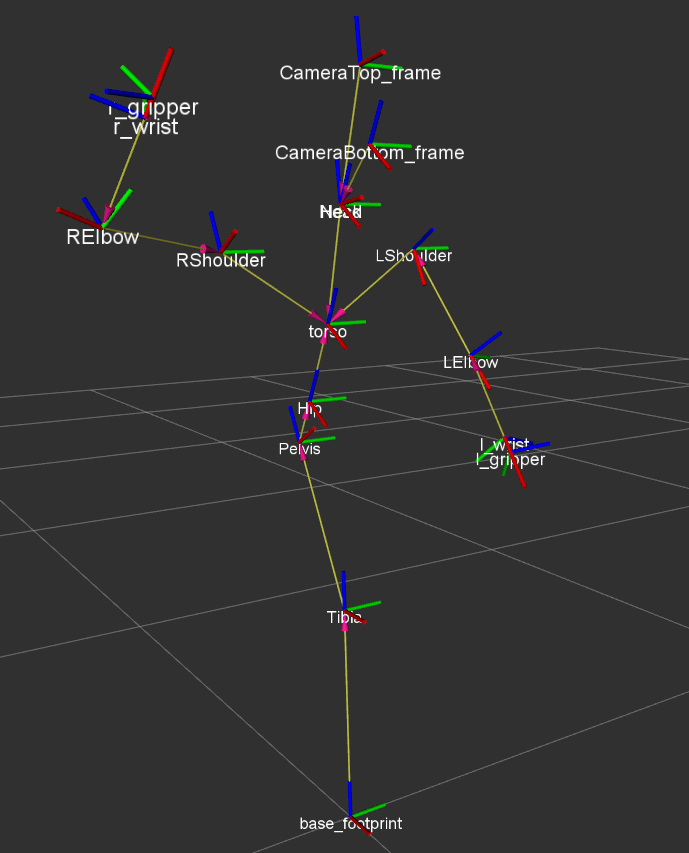
\includegraphics[width=\linewidth]{frames_pepper}
        \end{center}
        \vfill\columnbreak

        \begin{itemize}
            \item \textbf{frames}
            \item \textbf{forward kinematics}
            \item \textbf{inverse kinematics}
        \end{itemize}

    \end{multicols}
\end{frame}

\begin{frame}[plain]

    \begin{center}

        \textbf{Lots of sensors!}

        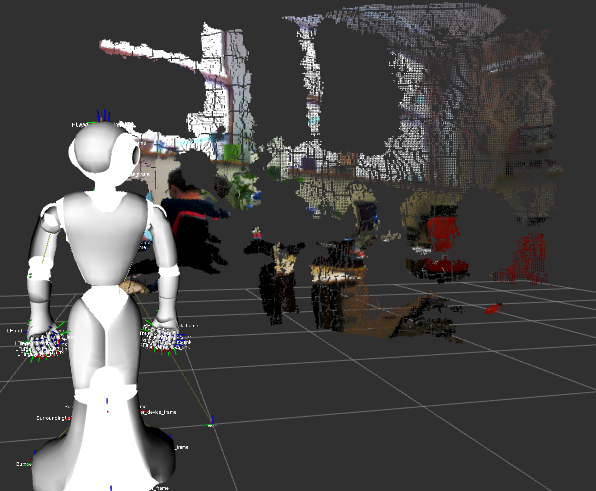
\includegraphics[width=0.6\linewidth]{rgbd_pepper}

    \end{center}

        \begin{itemize}
            \item \textbf{RGB-D cameras}, color + depth registration
            \item \textbf{Laserscans}
            \item \textbf{Sonars},...
        \end{itemize}

\end{frame}

\imageframe[color=black,caption=2D mapping!]{mapping_pepper}
\imageframe[color=black, caption=3D mapping!]{octomap_pepper}

\begin{frame}[plain]

    \begin{center}

        \textbf{Odometry is not good enough}

        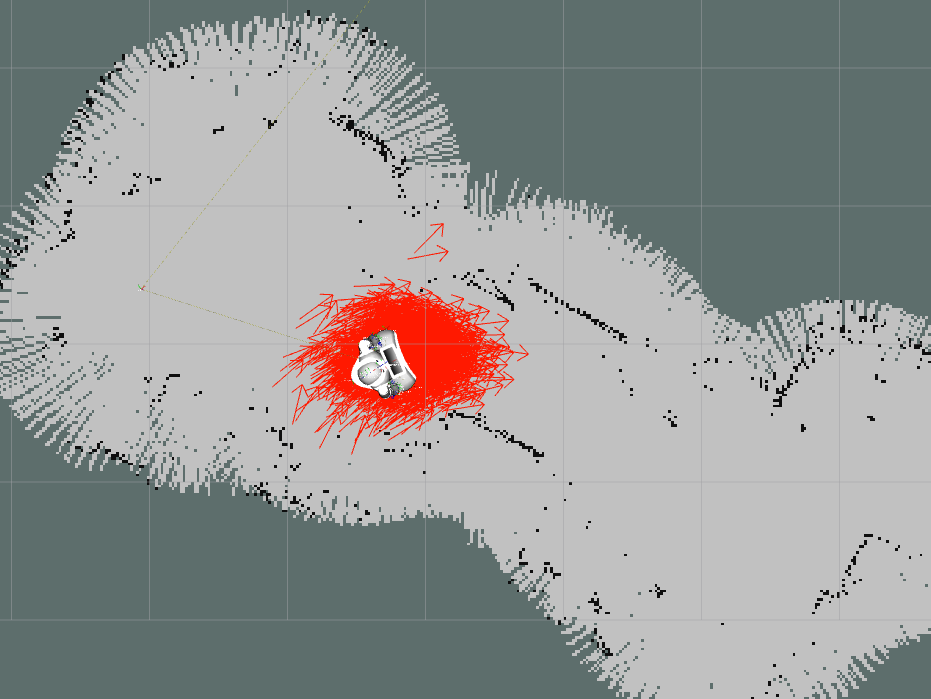
\includegraphics[width=0.6\linewidth]{localisation_pepper}

    \end{center}

        \begin{itemize}
            \item \textbf{SLAM} (Simultaneous Localization and Mapping)
            \item using \textbf{probabilistic reasoning} (Monte-Carlo localisation)
        \end{itemize}

\end{frame}

\imageframe[color=black,caption=Costmaps \& Motion planning]{motion_planning_pepper_rviz}

\begin{frame}[plain]

\begin{center}
    \textbf{Robotic middleware} to connects components together
    \vspace{3em}

\begin{tikzpicture}[
                    >=latex,
                    every edge/.style={->, draw, very thick},
                    service/.style={->, draw, very thick,dashed},
                    rosnode/.style={draw, font=\sf, node distance=0.5, rounded
                    corners, align=center, inner sep=5pt,fill=hriSec2Dark!50},
                    topic/.style={font=\tt, node distance=0.5, align=center, inner sep=5pt},
                    pic/.style={fill=none,draw=none}
                ]

    \path[use as bounding box] (-6,1) rectangle (6,-5);
    \node [rosnode] at (0,0) (node1) {node 1};
    \node [rosnode] at (4,-2) (node2) {node 2};
    \node [rosnode] at (-5,-4) (node3) {node 3};

        \node [topic] at (1,-2) (topic1) {/topic1};
        \node [topic] at (-1,-3) (topic2) {/topic2};
        \node [topic] at (-4,-2) (topic3) {/topic3};
        \path (node1) edge[bend left] node[label,right] {} (topic1);
        \path (node1) edge[bend right] node[label,left] {publishes} (topic2);
        \path (node3) edge[bend left] node[label,left] {} (topic3);
        \path (topic1) edge[bend right] node[label,below left] {subscribes} (node2);
        \path (topic2) edge[bend left] node[label,below] {} (node3);
        \path (topic2) edge[bend right] (node2);
        \path[->, dashed] ([yshift=2pt]node1.east) edge[bend left] node[label,above right] {action goal} ([xshift=2pt]node2.north) ;
        \path[->, dashed] ([xshift=-2pt]node2.north) edge[bend right] node[label,below left] {result} ([yshift=-2pt]node1.east);

        \node [rosnode,fill=hriSec3!50] at (-5,0) (roscore) {roscore};
        \path[dashed] (node1) edge[<->,very thin, bend right] node[label,above] {\tiny XML-RPC} (roscore);
        \path[dashed] (node2) edge[<->,very thin, bend right] node[label,above] {\tiny XML-RPC} (roscore);
        \path[dashed] (node3) edge[<->,very thin, bend left] node[label,above right] {\tiny XML-RPC} (roscore);


\end{tikzpicture}
\end{center}

\end{frame}


\begin{frame}[plain]{}
    Well, ROCO318 is over...

    \pause
    (oh no, I forgot about the autonomous chairs...)
\end{frame}


\videoframe[0.56]{figs/part1/NISSAN-ProPILOT-chair.mp4}


\begin{frame}{}
    \begin{center}
        \Large
        That's all, folks!\\[2em]
        \normalsize
        See you on Friday, 12:00\\[1em]
        Questions:\\
        Portland Square B316 or \url{severin.lemaignan@plymouth.ac.uk} \\[1em]

        Slides:\\ \href{https://github.com/severin-lemaignan/module-mobile-and-humanoid-robots}{\small github.com/severin-lemaignan/module-mobile-and-humanoid-robots}

    \end{center}
\end{frame}



\end{document}
